\documentclass[10pt,a4paper]{article}
\usepackage{amsmath}
\usepackage{amsfonts}
\usepackage{amssymb}
\usepackage{graphicx}
\usepackage[frenchb]{babel}
\usepackage[utf8x]{inputenc}
\graphicspath{{images/}}
\usepackage{parskip}
\usepackage{fancyhdr}
\usepackage{vmargin}
\usepackage{caption}
\usepackage{subcaption}
\usepackage{hyperref}

\setmarginsrb{3 cm}{2.5 cm}{3 cm}{2.5 cm}{1 cm}{1.5 cm}{1 cm}{1.5 cm}

\title{Travaux pratiques avec Weka}                             % Title
\author{Maxime De Wolf}                               % Author
\date{\today}                                           % Date

\makeatletter
\let\thetitle\@title
\let\theauthor\@author
\let\thedate\@date
\makeatother

\pagestyle{fancy}
\fancyhf{}
\rhead{\theauthor}
\lhead{\thetitle}
\cfoot{\thepage}

\begin{document}
   	
   	%%%%%%%%%%%%%%%%%%%%%%%%%%%%%%%%%%%%%%%%%%%%%%%%%%%%%%%%%%%%%%%%%%%%%%%%%%%%%%%%%%%%%%%%%
   	
   	\begin{titlepage}
   		\centering
   		\vspace*{0.5 cm}
   		
\includegraphics[scale = 0.75]{UMONS}\\[1.0 cm]   % University Logo
   		\textsc{\LARGE Université de Mons}\\[2.0 cm]   % University Name
   		\textsc{\large Datawarehousing and datamining}\\[0.5 cm]               % Course Name
   		\rule{\linewidth}{0.2 mm} \\[0.4 cm]
   		{ \huge \bfseries \thetitle}\\
   		\rule{\linewidth}{0.2 mm} \\[1.5 cm]
   		
   		\begin{minipage}{0.4\textwidth}
   			\begin{flushleft} \large
   				\emph{Auteur:}\\
   				\theauthor
   			\end{flushleft}
   		\end{minipage}~
   		\begin{minipage}{0.4\textwidth}
   			\begin{flushright} \large
                                 % Your Student Number
   			\end{flushright}
   		\end{minipage}\\[2 cm]
   		
   		{\large \thedate}\\[2 cm]
   		
   		\vfill
   		
   	\end{titlepage}
   	
   	%%%%%%%%%%%%%%%%%%%%%%%%%%%%%%%%%%%%%%%%%%%%%%%%%%%%%%%%%%%%%%%%%%%%%%%%%%%%%%%%%%%%%%%%%
   	
   	\tableofcontents
   	\newpage
   	
   	%%%%%%%%%%%%%%%%%%%%%%%%%%%%%%%%%%%%%%%%%%%%%%%%%%%%%%%%%%%%%%%%%%%%%%%%%%%%%%%%%%%%%%%%%
   	
   	\section{Weka: Tutoriel}
   	
	   	\subsection{Questions 17.1.9 et 17.1.10}
		   	Ces questions portent sur l'arbre de décision crée à partir du fichier \textit{iris.arff}. Voici donc l'arbre de décision obtenu:
		   	
		   	\begin{figure}[h]
		   		\begin{center}
		   			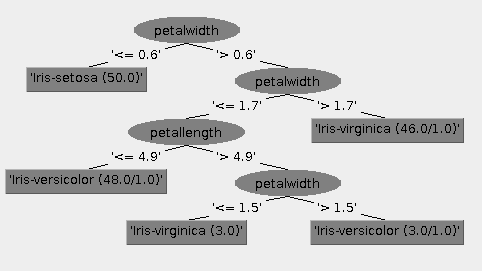
\includegraphics[width=0.3\linewidth]{IrisTree}
		   		\end{center}
		   		\caption{Arbre de décision du \textit{dataset iris.arff}}
		   		\label{fig-Iris-tree}
		   	\end{figure}
		   	
		   	\subsubsection*{Question 17.1.9}
			   	Cette question consiste à évaluer la qualité de cet arbre (Figure \ref{fig-Iris-tree}) grâce à différentes options de tests. Ici, on effectuera ces tests une première fois avec le \textit{dataset} complet et la $2^{e}$ fois avec la technique \textit{10-fold cross-validation}. Nous comparons ensuite les résultats obtenus sur base des 2 \textit{confusion matrix}:\\
	   			
	   			\begin{table}[h]
	   				\centering
	   				\caption{\textit{Confusion matrix} obtenues grâce à deux méthodes de test différentes}
					\begin{subtable}{0.4\textwidth}
						\centering
						\begin{tabular}{|c|c|c|l|}
							\hline
							a & b & c & \\ 
							\hline
							50 & 0 & 0 & a = Iris-setosa\\
							\hline
							0 & 49 & 1 & b = Iris-versicolor\\
							\hline
							0 & 2 & 48 & c = Iris-virginica\\
							\hline
						\end{tabular}
						\caption{\textit{Dataset} complet}
					\end{subtable}%
					\begin{subtable}{0.4\textwidth}
						\centering
						\begin{tabular}{|c|c|c|l|}
							\hline
							a & b & c & \\ 
							\hline
							49 & 1 & 0 & a = Iris-setosa\\
							\hline
							0 & 47 & 3 & b = Iris-versicolor\\
							\hline
							0 & 2 & 48 & c = Iris-virginica\\
							\hline
						\end{tabular}
						\caption{\textit{10-fold cross-validation}}
					\end{subtable}
	   			\end{table}
 
				 Nous remarquons que le test sur le \textit{dataset} complet classifie correctement $98\%$ des instances tandis que ce chiffre descend à $96\%$ avec le test \textit{10-fold cross-validation}. Tester le modèle avec le \textit{dataset} complet est une mauvaise idée car il donne une estimation optimiste de la qualité du modèle. En revanche, \textit{10-fold cross-validation} permet de se faire une bonne idée de la généralisation du modèle et offre donc une meilleure mesure de qualité.
				 
			\subsubsection*{Question 17.1.10}
			
				En observant la localisation de ces erreurs, nous remarquons que certaines instances de classe \textit{Iris-Verginica} ont des valeurs d'attributs équivalentes à celles d'instance de classe \textit{Iris-Versicolor}. Le modèle n'a donc aucune chance de les différencier si nous voulons éviter l'\textit{overfitting}. D'autre part, nous remarquons que l'instance de classe \textit{Iris-Setosa} qui a été mal identifier aurait dû être correctement classé selon l'arbre de décision final obtenu. 
		
		\subsection{Questions 17.2.4 à 17.2.11}
		
			\subsubsection*{Question 17.2.4}
				Le but de cette question est d'étudier la précision du classificateur \textit{5-nearest neighbor} en fonction des attributs utilisés lors de cette classification. Ici, nous exécutons cette algorithme sur le \textit{dataset glass.arff} et nous le test grâce à la technique \textit{10-fold cross-validation}. Les résultats ainsi obtenus sont résumés dans la table suivante:
				
				\begin{table}[h]
					\centering
					\caption{Précision obtenue en utilisant \textit{IBk} pour différents sous-ensemble d'attributs}
					\begin{tabular}{|c|c|c|}
						\hline
						Nombre d'attributs & Attribut retiré & Précision de la classification\\
						\hline
						9 & $\emptyset$ & 67.757 \\
						\hline
						8 & Si & 71.4953 \\
						\hline
						7 & Fe & 73.3645 \\
						\hline
						6 & Al & 73.3645 \\
						\hline
						5 & Na & 74.2991 \\
						\hline
						4 & Ba & 74.7664 \\
						\hline
						3 & K & 72.4299 \\
						\hline
						2 & Ca & 71.9626 \\
						\hline
						1 & Mg & 52.8037 \\
						\hline
						0 & RI & 35.514\\
						\hline
					\end{tabular}
				\end{table}
				
				Grâce à ce tableau, nous remarquons donc que la précision de \textit{IBk} sur le \textit{dataset} complet est de $67.757\%$ alors que nous obtenons une précision de $74.7664\%$ une fois que nous retirons les attributs \textit{Si, Fe, Al, Na, Ba} du \textit{dataset}. Ce qui nous donne un gain d'environ $7\%$ de précision.
			
			\subsubsection*{Question 17.2.5}
			
				Cette question demande de critiquer la pertinence de la précision maximum obtenue dans la question précédente. Ou, en d'autres mots, cette estimation est-elle biaisée ou non ?
				Etant donné que le test du modèle est effectué sur le \textit{dataset} d'entraînement, cette estimation est effectivement biaisée.
				
			\newpage
				
			\subsubsection*{Question 17.2.6}
				Cette question nous demande de constater l'effet du bruit sur un modèle construit grâce à \textit{IBk}. Pour ce faire, nous allons faire varier le pourcentage de bruits ainsi que la taille du voisinage dans les paramètres d'\textit{IBk}. Ainsi, une estimation de la précision sera calculé avec \textit{10-fold cross-validation}. Il est important de noter que ce test se fera sans les ajouts de bruits. Il n'y a donc présence de bruit que lors de la phase d'entraînement mais pas lors de la phase de test. La table suivante résume les résultat obtenus: 
			
				\begin{table}[h]
					\centering
					\caption{Effet du bruit sur la précision d'\textit{IBk}, en fonction de différentes tailles de voisinage}
					\label{tab-IBk-noise}
					\begin{tabular}{|c|c|c|c|}
						\hline
						Pourcentage de bruit & k = 1  & k = 3  & k = 5  \\
						\hline
						$0\%$ & $70.6\%$ & $72.0\%$ & $67.8\%$ \\
						\hline
						$10\%$ & $62.6\%$ & $69.6\%$ & $64.5\%$ \\
						\hline
						$20\%$ & $50.5\%$ & $63.1\%$ & $61.7\%$ \\
						\hline
						$30\%$ & $47.2\%$ & $58.4\%$ & $59.8\%$ \\
						\hline
						$40\%$ & $41.1\%$ & $54.7\%$ & $55.1\%$  \\
						\hline
						$50\%$ & $33.2\%$ & $44.4\%$ & $45.3\%$ \\
						\hline 
						$60\%$ & $27.1\%$ & $35.5\%$ & $35.5\%$ \\
						\hline 
						$70\%$ & $20.1\%$ & $28.5\%$ & $29.0\%$ \\
						\hline 
						$80\%$ & $14.0\%$ & $21.0\%$ & $21.0\%$ \\
						\hline 
						$90\%$ & $7.9\%$ & $13.6\%$ & $9.3\%$ \\
						\hline 
						$100\%$ & $4.7\%$ & $7.9\%$ & $7.5\%$ \\
						\hline 
					\end{tabular}
				\end{table}
				
			\subsubsection*{Question 17.2.7}
			
				Cette question nous demande de critiquer les résultats obtenues lors de la question précédente. Plus particulièrement, on nous demande l'effet qu'a une augmentation du bruit au niveau de la classe. La Table \ref{tab-IBk-noise} nous permet de constater que cette augmentation réduit la précision du classificateur \textit{k-nearest neighbor} et ce peu importe la valeur du k.
				
				\subsubsection*{Question 17.2.8}
				
				Cette question s'intéresse plutôt aux effets qu'a la modification de la valeur de k pour le classificateur \textit{k-nearest neighbor}. Dans la Table \ref{tab-IBk-noise} nous remarquons qu'augmenter la valeur de k rend le modèle obtenu plus robuste au bruit.\\
				
				En effet, nous remarquons que bien qu'il n'y ait pas de différence significative entre les modèles obtenus pour k = 3 et k = 5, ils sont plus résistants au bruit que ceux obtenus pour k = 1.
				
			\newpage
				
			\subsubsection*{Question 17.2.9}
				Pour cette question, nous devons comparer les classificateurs \textit{IBk} et \textit{J48} en fonction du pourcentage de l'ensemble d'apprentissage utilisé. Ces résultats sont encodés dans la table suivante:
			
				\begin{table}[h]
					\centering
					\caption{Variation de la précision du modèle en fonction de la taille de l'ensemble d'apprentissage pour \textit{IBk} et \textit{J48}}
					\label{tab-IBk-J48}
					\begin{tabular}{|c|c|c|}
						\hline
						Pourcentage de l'ensemble d'apprentissage & \textit{IBk} & \textit{J48}\\
						\hline
						$10\%$ & $52.8\%$ & $45.3\%$ \\
						\hline
						$20\%$ & $63.6\%$ & $53.3\%$ \\
						\hline
						$30\%$ & $60.3\%$ & $59.3\%$ \\
						\hline
						$40\%$ & $63.6\%$ & $65.0\%$ \\
						\hline
						$50\%$ & $62.6\%$ & $63.1\%$ \\
						\hline
						$60\%$ & $64.5\%$ & $69.2\%$ \\
						\hline
						$70\%$ & $65.9\%$ & $67.8\%$ \\
						\hline
						$80\%$ & $67.8\%$ & $70.1\%$ \\
						\hline
						$90\%$ & $67.3\%$ & $69.6\%$ \\
						\hline
						$100\%$ & $66.8\%$ & $68.2\%$ \\
						\hline
					\end{tabular}
				\end{table}
			
			\subsubsection*{Question 17.2.10}
		
			Cette question s'intéresse à l'effet de l'augmentation de nombre d'éléments de l'ensemble d'entraînement. Nous pouvons répondre à cette question grâce à la Table \ref{tab-IBk-J48}. Nous observons ainsi que plus l'ensemble d'entraînement est grand, plus la précision du modèle augmente jusqu'à un certain seuil où elle devient constante. Nous constatons que ce seuil se situe aux environs de $67\%$ pour \textit{IBk} et $69\%$ pour \textit{J48}.
		
			\subsubsection*{Question 17.2.11}
		
			On nous demande ici d'identifier laquelle des deux techniques -\textit{IBk} et \textit{J48}- est la plus affectée par l'augmentation de la taille de l'ensemble d'entraînement. En nous référant à la Table \ref{tab-IBk-J48}, nous observons que \textit{IBk} a une précision initiale de $52.8\%$ pour arriver finalement à une précision de $66.8\%$. La précision du modèle \textit{IBk} subit donc une variation de $14\%$. Pour \textit{J48}, la précision du modèle varie de $45.3\%$ à $68.2\%$ ce qui donne une variation de $22.9\%$. Comme le modèle \textit{J48} à une plus grande variation que \textit{IBk}, nous concluons que \textit{J48} est la technique la plus sensible à la taille de l'ensemble d'apprentissage.
			
		\subsection{Questions 17.3.1 à 17.3.11}
		
			\subsubsection*{Question 17.3.1}
			
			Pour résoudre cette question, nous utilisons le \textit{boundary visualizer} de \textit{Weka}. Cet outil sert à visualiser graphiquement les prédictions d'un modèle, dans notre cas, ce modèle est produit par le classificateur \textit{1R}. La Figure \ref{fig:iris:OneR} montre le résultat obtenu. Nous y voyons que la prédiction du modèle ne se fait uniquement qu'en fonction de la largeur des pétales (axe Y).
			
			\begin{figure}[h]
				\centering
				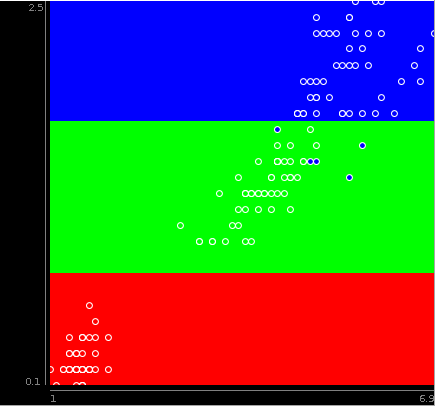
\includegraphics[width=.5\textwidth]{iris_OneR}
				\caption{Prédiction du type d'iris en fonction de la longueur des pétales (axe X) et de la largeur des pétales (axe Y) grâce au modèle 1R}
				\label{fig:iris:OneR}
			\end{figure}
			
			\subsubsection*{Question 17.3.2}
			
			Pour résoudre cette question, nous avons du jouer avec le paramètre \textit{minBucketSize} du classificateur \textit{1R}. Après avoir testé plusieurs valeurs, nous pouvons conclure que ce paramètre ne change pas les résultats obtenus lors de la question précédente (voir Figure \ref{fig:iris:OneR}).\\
			
			Nous pensons que c'est parce les valeurs que peuvent prendre la largeur des pétales (axe Y) varient entre $0.1$ et $2.5$. Il ne faut donc que 3 \textit{buckets} pour discrétiser ces valeurs. Etant donné le nombre d'instances de ce jeu de données, la valeur de \textit{minBucketSize} n'est utilisée que si elle n'est supérieure ou égale à 50. 50 est la valeur frontière car il y a 50 instances associés à chaque label.
			
			\subsubsection*{Question 17.3.3}
			
			On doit répondre à la question "Pourquoi n'y a-t-il pas plus de régions lorsque le \textit{bucket} a une petite valeur minimale ?". Cela s'explique car il s'agit d'une valeur minimale et donc, comme sur ce jeu de données on a relativement beaucoup d'instances par \textit{bucket}, la valeur de ce paramètre n'est pas prise en compte.
			
			\subsubsection*{Question 17.3.4}
			
			Le nombre minimum de région est 1 et la valeur minimum du paramètre \textit{minBucketSize} pour l'obtenir est 51. Cela peut s'expliquer simplement par le fait que chaque classe ne définit chacune que 50 instances.
			
			\subsubsection*{Question 17.3.5}
			
			En utilisant le classificateur \textit{IBK} avec k=1, nous obtenons la prédiction visible à la Figure \ref{fig:iris:IB1}. Comme expliqué dans l'énoncé, chaque point ne possède qu'une des trois couleurs (rouge, vert ou bleu) car k vaut 1 et donc, le modèle ne prédit pas un point pouvant appartenir à plusieurs classe.\\
			
			Nous remarquons néanmoins une zone du graphique qui fait exception à cela car sa couleur est une nuance de bleu (et pas totalement bleu). Nous pouvons justifier cela car il existe plusieurs instances qui ont les même longueur et largeur de pétale mais qui sont associés à des classes différentes. La zone possédant une couleur nuancée est en fait la zone qui contient ces instances.   
			
			\begin{figure}[h]
				\centering
				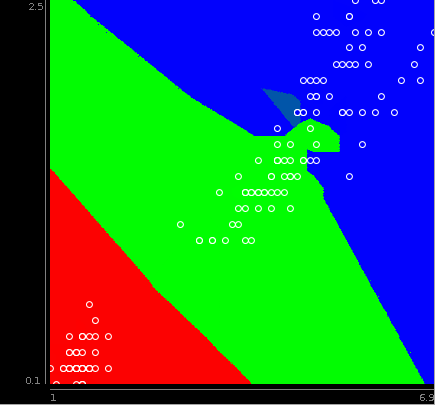
\includegraphics[width=.5\textwidth]{iris_IB1}
				\caption{Prédiction du type d'iris en fonction de la longueur des pétales (axe X) et de la largeur des pétales (axe Y) grâce au modèle IBK (avec k=1)}
				\label{fig:iris:IB1}
			\end{figure}
			
			\subsubsection*{Question 17.3.6}
			
			En augmentant les valeurs du paramètre k, nous remarquons que les zones de la prédiction sont de plus en plus nuancées comme nous le montre la Figure \ref{fig:iris:IB5-10}.
			
			\begin{figure}[!]
				\centering
				\begin{subfigure}{.5\textwidth}
					\centering
					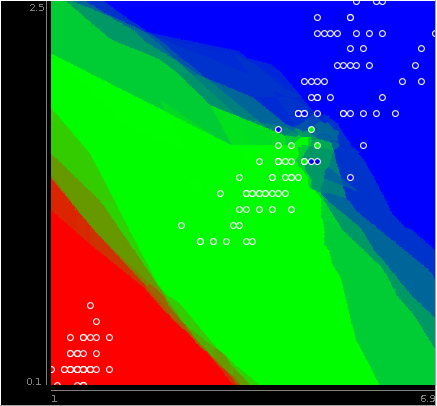
\includegraphics[width=.9\textwidth]{iris_IB5}
					\caption{k=5}
				\end{subfigure}%				
				\begin{subfigure}{.5\textwidth}
					\centering
					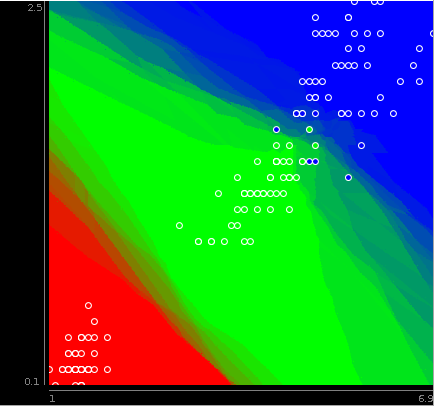
\includegraphics[width=.9\textwidth]{iris_IB10}
					\caption{k=10}
				\end{subfigure}

				\caption{Prédiction du type d'iris en fonction de la longueur des pétales (axe X) et de la largeur des pétales (axe Y) grâce au modèle IBK}
				\label{fig:iris:IB5-10}
			\end{figure}
			
			\subsubsection*{Question 17.3.7}
			
			Effectivement, comme le montre la Figure \ref{fig:iris:NaiveBayes}, la prédiction donnée par le modèle \textit{NaïveBayes} a un \textit{pattern} très différent des prédictions précédemment obtenues.\\
			
			Nous pouvons expliquer ce \textit{pattern} par le fait que \textit{NaïveBayes} base sa prédiction par rapport à la probabilité d'appartenir à une classe selon les valeurs X et Y d'une instance. Cela donne donc ce motif quadrillé.\\
			
			La couleur de chaque zone est ensuite calculée en fonction de la "couleur" des instances qu'elle contient ainsi qu'aux autres zones "proche". Comme les instances de notre jeu de données se situent surtout sur la diagonale montante, nous obtenons un motif symétrique.	
			
			\begin{figure}[!]
				\centering
				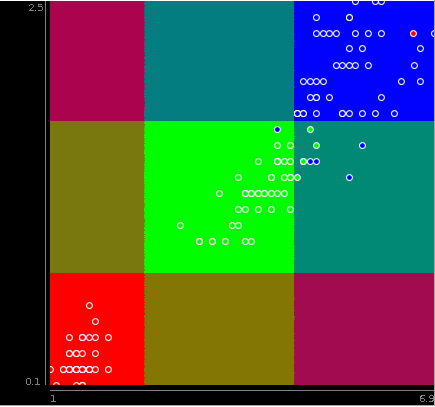
\includegraphics[width=.5\textwidth]{iris_NaiveBayes}
				\caption{Prédiction du type d'iris en fonction de la longueur des pétales (axe X) et de la largeur des pétales (axe Y) grâce au modèle NaïveBayes}
				\label{fig:iris:NaiveBayes}
			\end{figure}
			
			\subsubsection*{Question 17.3.8}
			
			Le modèle \textit{JRip} nous donne la prédiction visible à la Figure \ref{fig:iris:JRip}. Nous pouvons y voir que le modèle fait ses prédictions en fonctions de la longueur des pétales (axe X) sauf pour les classes \textit{iris-versicolor} où la largeur des pétales intervient également.\\
			
			Un petit coup d'œil dans l'\textit{explorer} de \textit{Weka} nous permet de savoir quelles sont les règles de prédiction utilisées par \textit{JRip}. Ces règles sont les suivantes:
			
			\begin{itemize}
				\item (petallength $\le$ 1.9) $\implies$ class=Iris-setosa
				\item (petalwidth $\le$ 1.6) and (petallength $\le$ 4.9) $\implies$ class=Iris-versicolor
				\item otherwise class=Iris-virginica
			\end{itemize}   
			
			\begin{figure}[h]
				\centering
				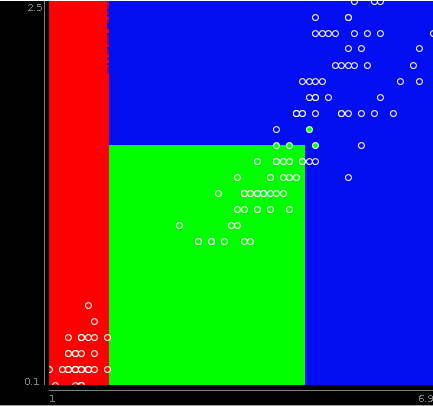
\includegraphics[width=.5\textwidth]{iris_JRip}
				\caption{Prédiction du type d'iris en fonction de la longueur des pétales (axe X) et de la largeur des pétales (axe Y) grâce au modèle JRip}
				\label{fig:iris:JRip}
			\end{figure}
			
			\subsubsection*{Question 17.3.9}
			
			Les règles utilisées par \textit{JRip} lors de la question précédente donnent de bonnes prédictions uniquement si elles sont exécutées dans le bon ordre. Voici un ensemble de règles équivalentes dont le résultat ne dépend pas de l'ordre dans lesquelles on les exécutent:
			
			\begin{itemize}
				\item (petallength $\le$ 1.9) $\implies$ class=Iris-setosa
				\item (petalwidth $\le$ 1.6) and (1.9 $<$ petallength $\le$ 4.9) $\implies$ class=Iris-versicolor
				\item (1.9 $<$ petallength) and (1.6 $<$ petalwidth) or (4.9 $<$ petallength) $\implies$ Iris-virginica
			\end{itemize}
			
			\subsubsection*{Question 17.3.10}
			
			La Figure \ref{fig:iris:J48} montre la prédiction suivant le modèle \textit{J48}. Sans surprise, nous pouvons voir que ce modèle découpe des zones soit selon l'axe X, soit selon l'axe Y, c'est pour cela qu'aucune zone n'est délimitée par un segment diagonal.\\
			
			Nous pouvons y voir une zone dont la couleur est une nuance de bleu et de vert. Cela vient du fait que l'arbre du modèle \textit{J48} a subi un élagage afin d'éviter un \textit{overfit} des données. Cette zone contient donc des instances appartenant à des classes différentes.\\
			
			La Figure \ref{fig:iris:J48:tree} montre l'arbre généré par J48 qui est utilisé pour faire les prédictions.
			
			\begin{figure}[h]
				\centering
				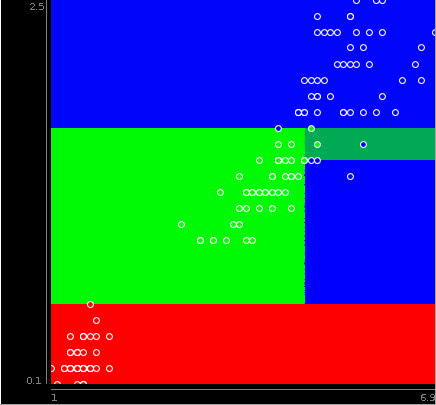
\includegraphics[width=.5\textwidth]{iris_J48}
				\caption{Prédiction du type d'iris en fonction de la longueur des pétales (axe X) et de la largeur des pétales (axe Y) grâce au modèle J48}
				\label{fig:iris:J48}
			\end{figure}
			
			\begin{figure}[h]
				\centering
				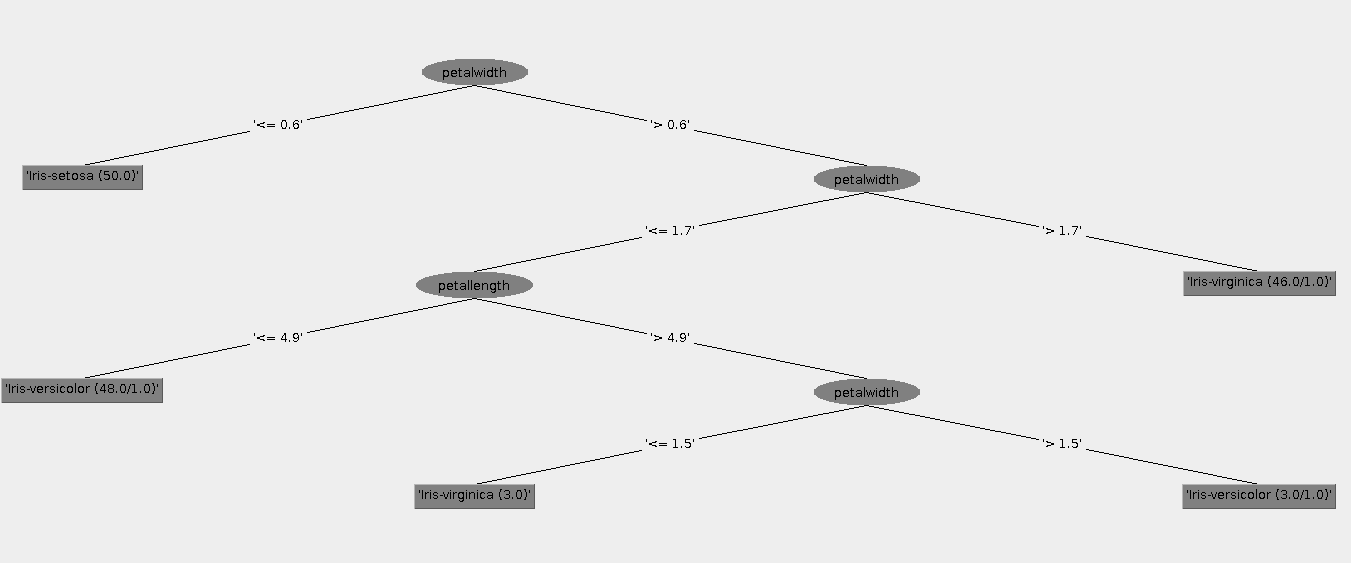
\includegraphics[width=.8\textwidth]{iris_J48_tree}
				\caption{Arbre généré par J48 afin de prédire le type d'iris}
				\label{fig:iris:J48:tree}
			\end{figure}
   	
   	
		   	\subsubsection*{Question 17.3.11}
		   	
		   	Pour résoudre cette question, nous devons jouer avec les arguments du modèle \textit{J48} afin d'obtenir 3, 2, puis une zone dans les prédictions. La Figure \ref{fig:iris:J48:zones} résume les résultats obtenus.
		   	
		   	\begin{figure}[!]
		   		\centering
		   		\begin{subfigure}{.333\textwidth}
		   			\centering
		   			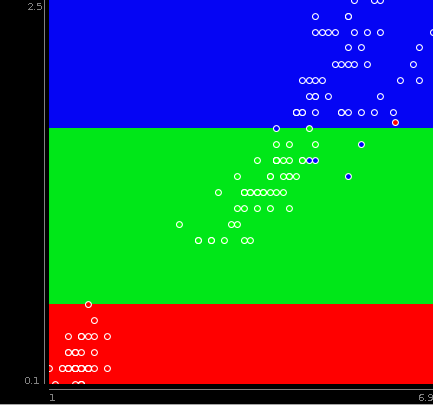
\includegraphics[width=.9\textwidth]{iris_J48_3zones}
		   			\caption{7 à 49 instances par feuilles}
		   		\end{subfigure}%				
		   		\begin{subfigure}{.333\textwidth}
		   			\centering
		   			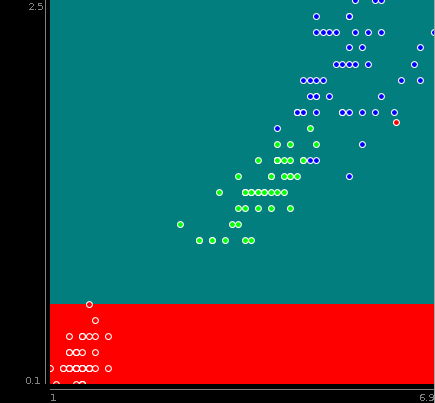
\includegraphics[width=.9\textwidth]{iris_J48_2zones}
		   			\caption{50 à 75 instances par feuilles}
		   		\end{subfigure}%
		   		\begin{subfigure}{.333\textwidth}
		   			\centering
		   			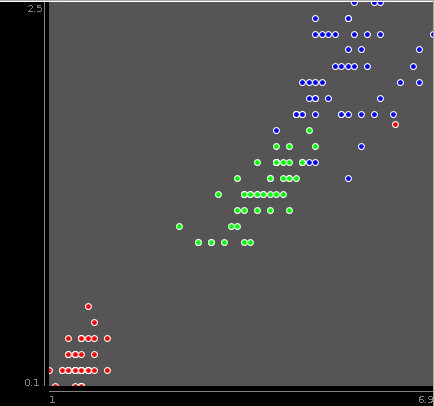
\includegraphics[width=.9\textwidth]{iris_J48_1zone}
		   			\caption{76 à 150 instances par feuilles}
		   		\end{subfigure}
		   		
		   		\caption{Variation du nombre de zones des prédictions du jeu de données \textit{Iris.arff} en fonction du paramètre \textit{minNumObj} de J48}
		   		\label{fig:iris:J48:zones}
		   	\end{figure}
		   	
		\subsection{Questions 17.4.1 à 17.4.4 + question 17.4.8}
		
			\subsubsection*{Question 17.4.1}
			
			Cette question porte sur la discrétisation non-supervisée des données. Il nous est donc demandé de discrétiser les données du fichier \textit{glass.arff} selon deux méthodes différentes : \textit{equal-width} et \textit{equal-frequency}. La Figure \ref{fig:glass:disc} montre les résultats ainsi obtenus.\\
			
			La méthode \textit{equal-width} discrétise les données en créant des intervalles de mêmes longueurs. Il est donc normal que nous voyons apparaître de gros écart de "population" entre les différents intervalles.\\
			
			La méthode \textit{equal-frequency} discrétise les données en créant des intervalles peuplés plus ou moins de la même façon. Il est donc normal que les écarts  de "population" entre intervalles sont très petits. Nous voyons tout de même quelques intervalles ayant de gros écarts avec les autres. Cela s'explique car ces pics sont causés par un grand nombre d'instances ayant la même valeur d'attribut. Il est donc normal qu'il soit impossible de placer ces instances dans des intervalles différents.
			
			\begin{figure}[h]
				\centering
				\begin{subfigure}{.5\textwidth}
					\centering
					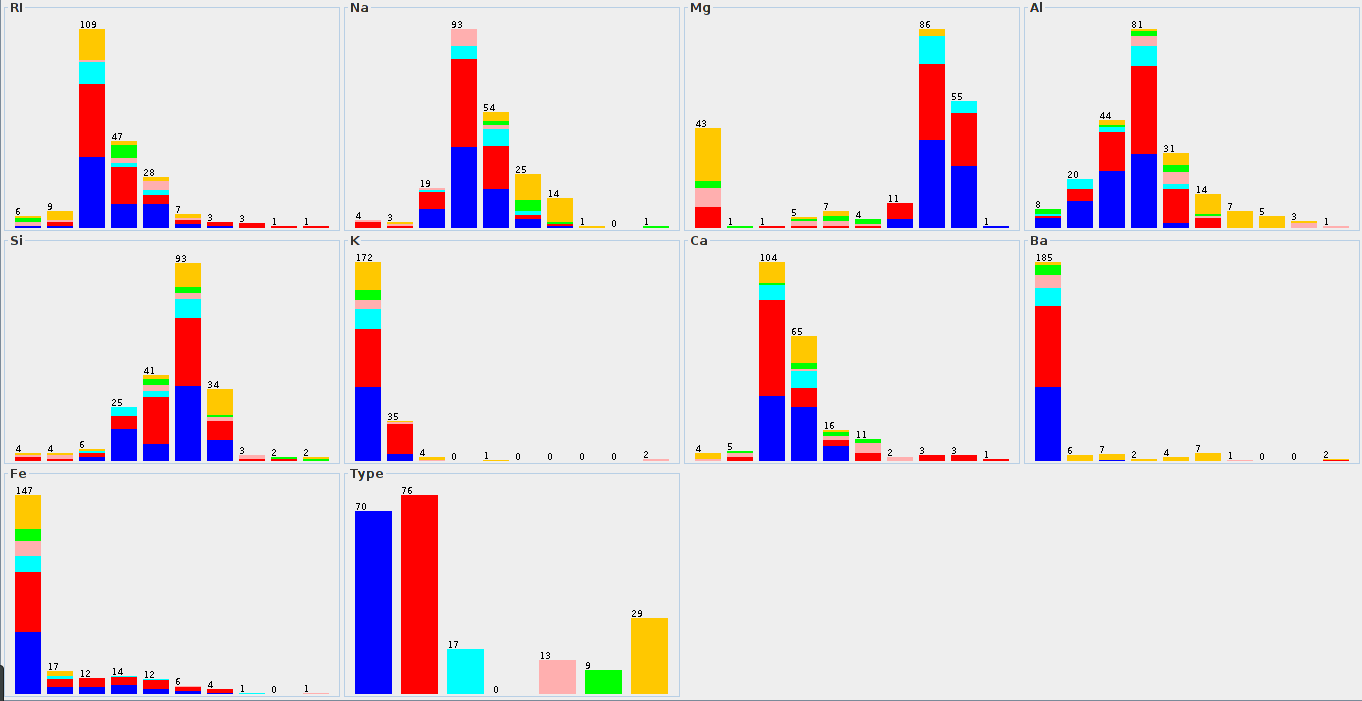
\includegraphics[width=.9\textwidth]{glass_disc_width}
					\caption{méthode \textit{equal-width}}
				\end{subfigure}%				
				\begin{subfigure}{.5\textwidth}
					\centering
					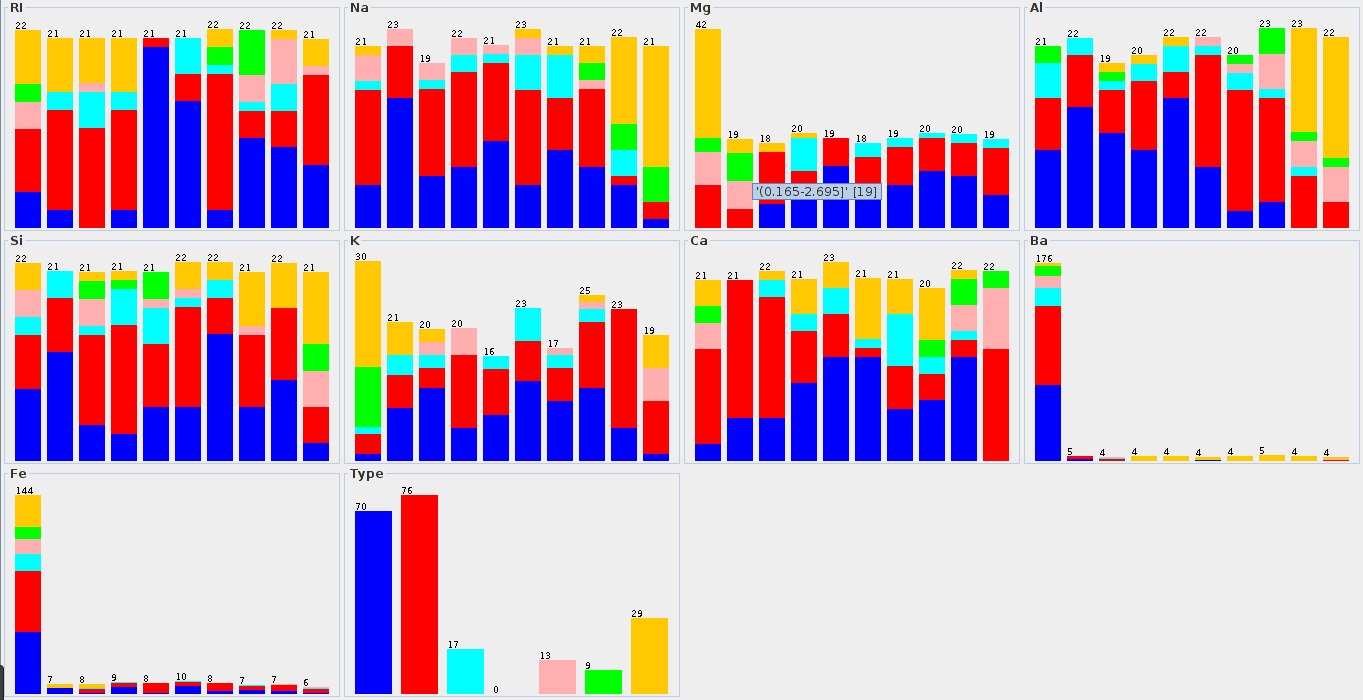
\includegraphics[width=.9\textwidth]{glass_disc_freq}
					\caption{méthode \textit{equal-frequency}}
				\end{subfigure}
				
				\caption{Discrétisation du jeu de données \textit{glass.arff} suivant 2 méthodes non-supervisées différentes}
				\label{fig:glass:disc}
			\end{figure}
			
			\subsubsection*{Question 17.4.2}
			
			La figure \ref{fig:iris:disc} montre le résultat de la discrétisation supervisée du fichier \textit{iris.arff}. Cette méthode permet de mettre en évidence les attributs les plus appropriés afin d'effectuer une classification. Ici, nous remarquons que l'attribut \textit{petalwidth} est un bon candidat pour tenter une classification. Cela conforte les résultats obtenus pour répondre aux questions du chapitre 17.3.
			
			\begin{figure}[h]
				\centering
				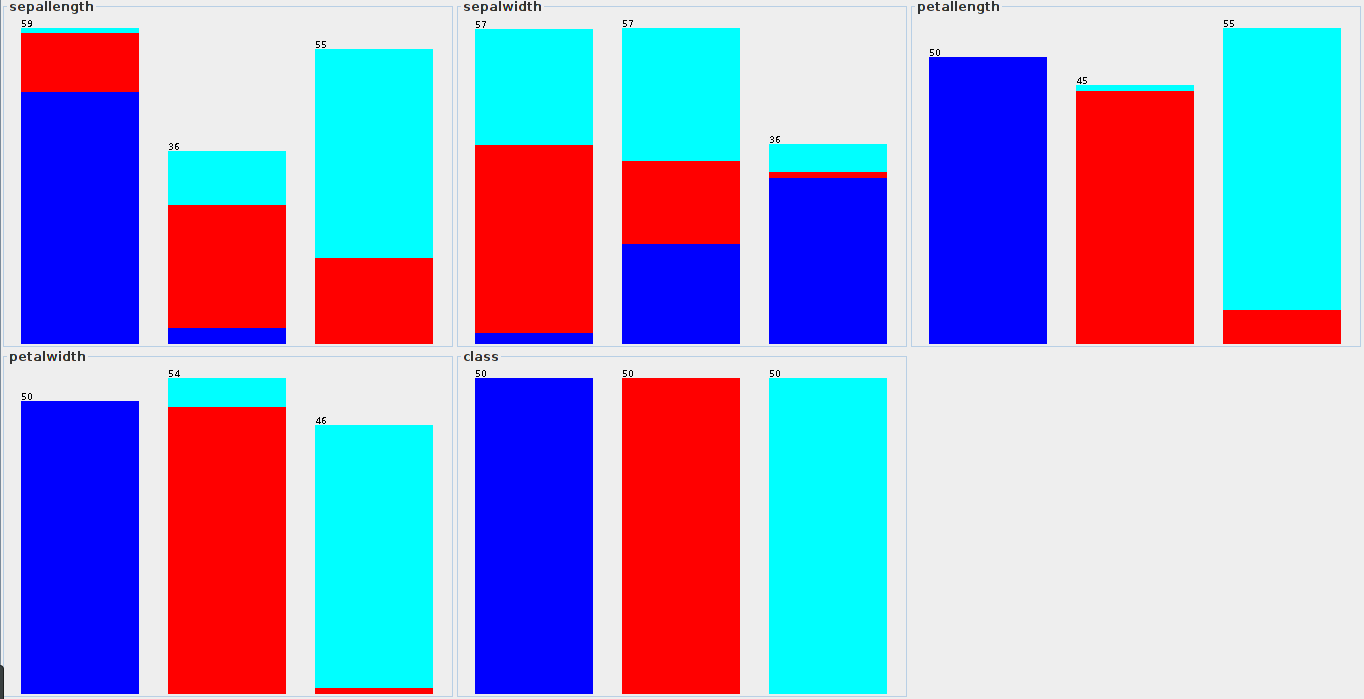
\includegraphics[width=.8\textwidth]{iris_disc}
				\caption{Discrétisation supervisée du fichier \textit{iris.arff}}
				\label{fig:iris:disc}
			\end{figure}
			
			
			\subsubsection*{Question 17.4.3}
			
			Cette question demande la même chose que la précédente sauf qu'on utilise cette fois le fichier \textit{glass.arff}. Nous remarquons que certains attributs ne comptent qu'un seul intervalle. Ces attributs (\textit{Fe} et \textit{Si}) sont en fait de très mauvais candidats pour effectuer une classification comme nous l'avons déjà remarqué pendant la question 17.2.4. 
			
			\begin{figure}[h]
				\centering
				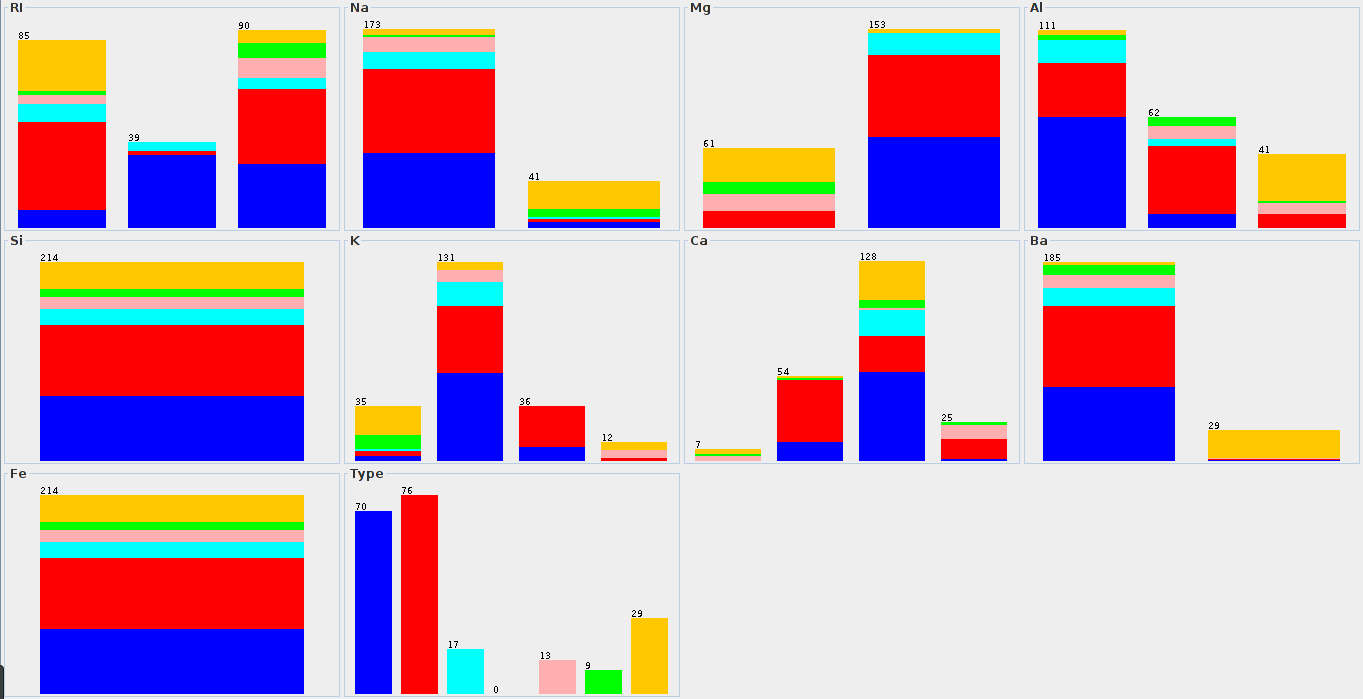
\includegraphics[width=.8\textwidth]{glass_disc_sup}
				\caption{Discrétisation supervisée du fichier \textit{glass.arff}}
				\label{fig:glass:disc:sup}
			\end{figure}
			
			
			\subsubsection*{Question 17.4.4}
			
			Pour cette question, nous effectuons la même manipulation qu'à la question précédente sauf que nous mettons le paramètre \textit{makeBinary} du filtre à vrai. Nous remarquons alors que ce paramètre sert à ne créer que 2 intervalles maximum par attribut quitte à créer de nouveaux attributs pour stocker les intervalles excédants. Nous pouvons avoir un aperçu de cette manipulation grâce à la Figure \ref{fig:glass:disc:bin}.
			
			\begin{figure}[h]
				\centering
				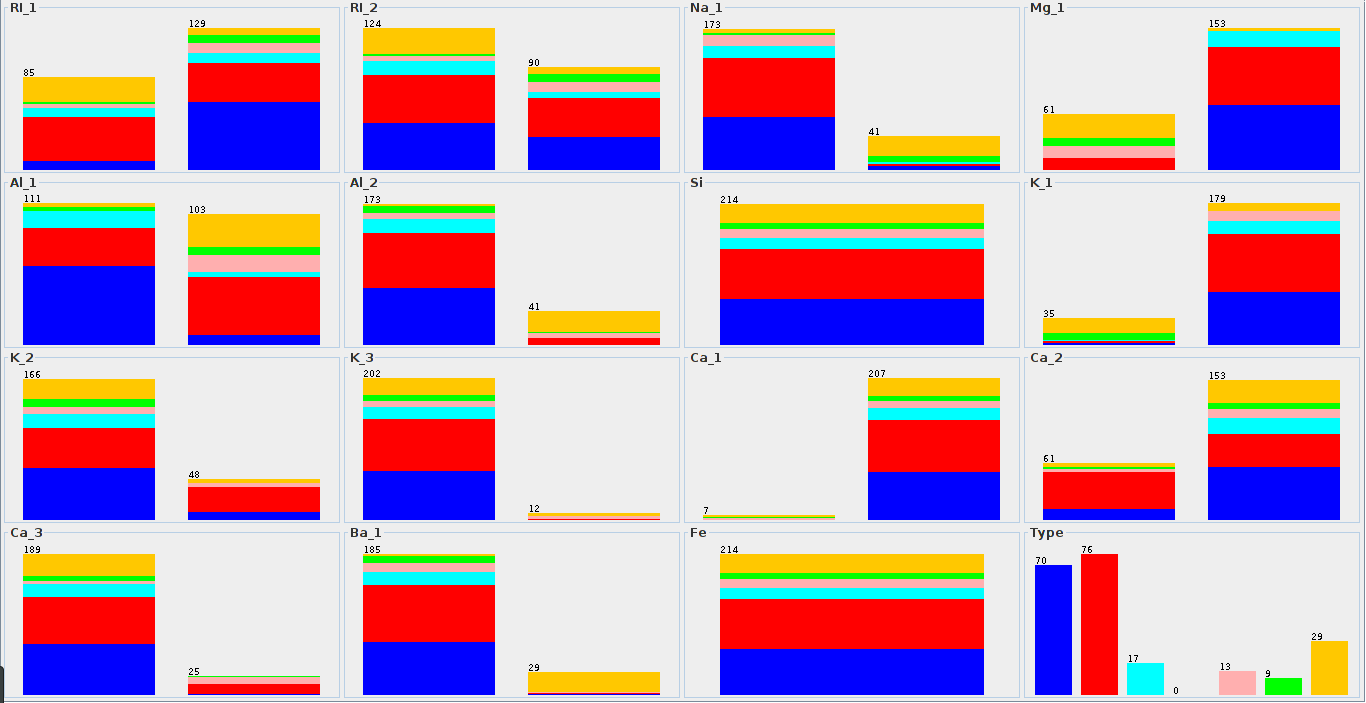
\includegraphics[width=.8\textwidth]{glass_disc_bin}
				\caption{Discrétisation supervisée du fichier \textit{glass.arff} avec le paramètre \textit{makeBinary} à vrai}
				\label{fig:glass:disc:bin}
			\end{figure}
			
			\subsubsection*{Question 17.4.8}
			
			Pour cette question, nous devions trouver les 4 attributs les plus pertinents dans le but d'une classification. Nos résultats sont les suivants par ordre décroissant de pertinence:
			
			\begin{enumerate}
				\item \textit{wage-increase-first-year}
				\item \textit{wage-increase-second-year}
				\item \textit{statutory-holidays}
				\item \textit{contribution-to-dental-plan}
			\end{enumerate}
			
		\subsection{Questions 17.5.1 à 17.5.4 + question 17.5.6}
		
			\subsubsection*{Question 17.5.1}
			
			Pour résoudre cette question, nous commençons par créer un document texte sur lequel nous appliquerons le filtre \textit{StringToWordVector}. Le document texte que nous avons créer contient les mêmes données que la Table \ref{tab:oil:training}.\\
			
			Ce filtre créer un jeu de données à partir de notre document texte. Il créer un attribut par mot, soit un total de 34 pour notre exemple. Ensuite, nous mettons le paramètre \textit{minTermFreq} de ce filtre à 2. Cela implique qu'il ne crée un nouvel attribut que pour un mot seulement si il apparaît au moins 2 fois dans le texte.
				
			\begin{table}[h]
				\centering
				\caption{Document d'apprentissage}
				\label{tab:oil:training}
				\begin{tabular}{|c c|}
					\hline
					\textbf{Document texte} & \textbf{Classification}\\
					The price of crude oil has increased significantly & yes\\
					Demand for crude oil outstrips supply & yes\\
					Some people do not like the flavor of olive oil & no\\
					The food was very oily & no\\
					Crude oil is in short supply & yes\\
					Use a bit of cooking oil in the frying pan & no\\
					\hline
				\end{tabular}
			\end{table}
				
			\subsubsection*{Question 17.5.2}
			
			Nous utilisons ces données fraîchement récoltées afin de créer un arbre de décision grâce à \textit{J48}. La Figure \ref{fig:text:training:tree} nous montre cet arbre.
			
			\begin{figure}[h]
				\centering
				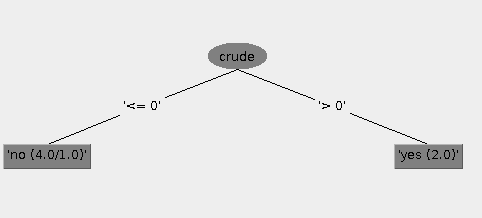
\includegraphics[width=.5\textwidth]{text_tree}
				\caption{Arbre de classification produit par \textit{J48}}
				\label{fig:text:training:tree}
			\end{figure}
			 
			\subsubsection*{Question 17.5.3}
			
			Nous testons ensuite cet arbre sur un jeu de données extrait d'un autre fichier texte. Ce fichier contient les mêmes données que la Table \ref{tab:oil:test}. Ce modèle nous donne les prédictions suivantes par ordre d'apparition dans la Table \ref{tab:oil:test}:
			
			\begin{enumerate}
				\item \textit{yes}      
				\item \textit{no}
				\item \textit{no}
				\item \textit{no}  
			\end{enumerate}
			
			Nous remarquons que ce modèle est cohérent même si sa troisième prédiction aurait du être \textit{yes}. Cela est sûrement dû au fait que l'ensemble d'entraînement est très petit.
			
			\begin{table}[h]
				\centering
				\caption{Document test}
				\label{tab:oil:test}
				\begin{tabular}{|c c|}
					\hline
					\textbf{Document texte} & \textbf{Classification}\\
					Oil platforms extract crude oil & ?\\
					Canola oil is supposed to be healthy & ?\\
					Iraq has significant oil reserves & ?\\
					There are different types of cooking oil & ?\\
					\hline
				\end{tabular}
			\end{table}
			
			\subsubsection*{Question 17.5.4}
			
			  Pour cette question, nous devons construire deux modèles en utilisant \textit{J48} et \textit{NaiveBayesMultinomial} pour deux jeux de données textuelles. Le premier de ces deux jeu de données a pour but d'identifier les textes qui parlent de maïs (\textit{ReutersCorn-train.arff}) tandis que le but du second est d'identifier les textes qui parlent de graines (\textit{ReutersGrain-train.arff}).\\
			  
			  La Table \ref{tab:corn} résume les résultats obtenus pour les deux classificateurs sur le premier jeu de données. Nous voyons que \textit{J48} est meilleur que \textit{NaiveBayesMultinomial} sur tous les plans. Il est donc évident que pour ce jeu de données, \textit{J48} est le classificateur que nous choisirions.\\ 
			  
			  \begin{table}[h]
			  	\centering
			  	\caption{Résultats des deux modèles entraînés sur \textit{ReutersCorn-train.arff} et testés sur \textit{ReutersCorn-test.arff}}
			  	\label{tab:corn}
		  		\begin{tabular}{|c|c|c|c|}
		  			\hline
		  			&Instances bien  & Précision & \textit{Recall}\\
		  			& classifiées  &  & \\ 
		  			\hline
		  			\textit{J48} & $97.4 \%$ & $97.3\%$ & $97.4\%$ \\
		  			\hline
		  			\textit{NaiveBayesMultinomial}& $93.7\%$ & $96.4\%$ & $93.7\%$ \\
		  			\hline
		  		\end{tabular}
			  \end{table}
			  
			  La Table \ref{tab:grain} montre les résultats des deux classificateurs sur le second jeu de données. Ici encore nous voyons que \textit{J48} est le meilleur des deux classificateurs. Toutefois, nous remarquons que \textit{NaiveBayesMultinomial} a une meilleure précision en moyenne. Cela veut dire que le modèle fait peu d'erreur lorsqu'il doit prédire la classe d'une instance. Cependant, il s'agit là d'une moyenne. En effet, en regardant les résultats de plus près, nous remarquons que ce modèle à en fait une très mauvaise précision ($21.4 \%$) pour ce qui est de repérer les textes qui parlent de graines. Cela conforte donc notre choix de \textit{J48}.
			  
			  \begin{table}[h]
			  	\centering
			  	\caption{Résultats des deux modèles entraînés sur \textit{ReutersGrain-train.arff} et testés sur \textit{ReutersGrain-test.arff}}
			  	\label{tab:grain}
			  	\begin{tabular}{|c|c|c|c|}
			  		\hline
			  		&Instances bien  & Précision & \textit{Recall}\\
			  		& classifiées  &  & \\ 
			  		\hline
			  		\textit{J48} & $94.5 \%$ & $96.2\%$ & $94.5\%$ \\
			  		\hline
			  		\textit{NaiveBayesMultinomial}& $86.3\%$ & $96.5\%$ & $86.3\%$ \\
			  		\hline
			  	\end{tabular}
			  \end{table}
			  
			  \subsubsection*{Question 17.5.6}
			  
			  La Table \ref{tab:text:ROC} montre les valeurs de \textit{ROC} des deux classificateurs sur les deux jeux de données. Contrairement aux résultats précédemment obtenus, \textit{NaiveBayesMultinomial} apparaît comme étant le meilleur classificateur pour ce problème.
			  
			  \begin{table}[h]
			  	\centering
			  	\caption{Récapitulatif des valeurs \textit{ROC} pour les 2 classificateurs et les 2 jeux de données}
			  	\label{tab:text:ROC}
			  	\begin{tabular}{|c|c|c|}
			  		\hline
			  		& Maïs & Graines \\
			  		\hline
			  		\textit{J48} & $69.4\%$ & $90.3\%$\\
			  		\hline
			  		\textit{NaiveBayesMultinomial} & $95.2\%$ & $96.5\%$\\
			  		\hline
			  	\end{tabular}
			  \end{table}
   	
   	\section{CoIL Challenge 2000}
   	
	   	\subsection{Description du problème}
	   	
		   	Le problème consiste à concevoir un modèle capable de détecter les personnes potentiellement intéressées par la souscription d'une assurance caravane. Le but de cette tâche est d'envoyer une publicité ciblée sur ces personnes afin de réduire les coûts de celle-ci. Nous nous limiterons donc à l'envoie de 800 de ces publicités.\\
		   	
		\subsection{Description des données}
		   	
		   	Pour concevoir ce modèle, nous possédons un fichier d'entraînement contenant les données "historiques" de 5822 personnes dont 348 ($\pm6\%$) possèdent une assurance caravane.\\
		   	
		   	Nous possédons également un fichier contenant les données de 4000 personnes parmi lesquelles nous aimerions envoyer les 800 courriers publicitaires. Nous nous attendons à ce que la même proportion de ces personnes soient intéressée par une assurance caravane que dans notre fichier "historique". Nous estimons donc que $6\%$ de ces 4000 personnes ($\pm240$) soient intéressées.
		   	
		\subsection{Mesures importantes}
		
			Afin de repérer au mieux les personnes intéressées par l'assurance caravane, notre modèle doit maximiser la mesure \textit{recall} afin de trouver un maximum de ces personnes. Nous devons également veiller à ce que la mesure \textit{precision} de notre modèle ne soit pas trop mauvaise afin de ne pas dépasser les 800 courriers publicitaires à envoyer.
			
		\subsection{Pré-traitement des données}
		
			\subsubsection*{Extraction des données}
			
				Dans un premier temps, nous devons convertir les fichiers de données en format compatible pour le logiciel \textit{Weka}. Pour ce faire, nous utilisions un petit programme \textit{Python} écrit par un autre élève: Nico Salamone.
				
			\subsubsection*{Sélection d'attributs}
			
				Afin de faire une sélection correcte des attributs du jeu de données, nous essayons plusieurs évaluateurs d'attributs afin d'être sûr de choisir la meilleure sélection d'attributs. Dans notre cas nous choisissons le modèle \textit{NaiveBayes} pour évaluer les sélections. Nous évaluerons l'efficacité d'une sélection selon les valeurs \textit{precision} et \textit{recall} de la classification pour la classe qui nous intéresse. La Table \ref{tab:select} résume les résultats obtenus pour les différentes sélections effectuées.
				
				Vous trouverez ci-dessus un détail sur les différents évaluateurs d'attributs testés. 
				\\
				
				Dans un premier temps nous effectuons la classification sur la totalité des attributs afin d'avoir un point de comparaison. Nous lançons donc le test sur les 85 attributs.
				
				Ensuite, nous testons l'évaluateur \textit{CfsSubsetEval} qui est l'évaluateur par défaut. Il sélectionne les attributs suivants: \textbf{25,42,43,44,47,59,61,64,68,82}. Comme le montre la Table \ref{tab:select}, les résultats obtenus sont très médiocre.
				
				L'évaluateur \textit{ConsistencySubsetEval} est légèrement meilleur mais n'est toujours pas satisfaisant. Il sélectionne les attributs suivant: \textbf{1,3,4,6,16,21,23,24,29,30,32,37,40,44,47,54,59,61,64,68}.
				
				Nous avons effectué plusieurs tests avec l'évaluateur \textit{GainRatioAttributeEval}. D'abord, nous avons sélectionné les attributs qui un ratio de gain supérieur à $0.01$. Cela nous a donné la sélection suivante: \textbf{82,61,47,85,64,68,86}. Malheureusement, une fois encore les résultats ne sont pas satisfaisant.\\
				Nous avons ensuite sélectionné les attributs dont le ratio de gain est supérieur à $0$. Cela nous a donc donné la sélection suivante: \textbf{82,61 ,47 ,85 ,64 ,68 ,25 ,19 ,59 ,42 ,37 ,65 ,43 ,44 ,30 ,31 ,18 ,54 ,75 ,10 ,34 ,39 ,12 ,80 ,5 ,16 ,32 ,1 ,29 ,28 ,21 ,40 ,22 ,24 ,23 ,35 ,36 ,13 ,2 ,6 ,3 ,4 ,86}. Cette sélection donne de bons résultats mais sont toujours inférieur aux résultats obtenus en sélectionnant la totalité des attributs.
				
				Nous avons également testé d'autres évaluateurs mais nous ne les avons pas mentionné car ils sélectionnaient soit aucun soit tout les attributs.
				
				\begin{table}[h]
					\centering
					\caption{Résultats des différentes sélections effectuées}
					\label{tab:select}
					\begin{tabular}{|c|c|c|}
						\hline
						& \textit{Precision} & \textit{Recall}\\
						\hline
						Pas de sélection & $13.6\%$& $48.6\%$\\
						\hline
						\textit{CfsSubsetEval} & $23.8\%$ & $10.9\%$ \\
						\hline
						\textit{ConsistencySubsetEval} & $19.8\%$ & $28.2\%$\\
						\hline
						\textit{GainRatioAttributeEval} $>0.01$ & $24.3\%$ & $7.8\%$ \\
						\hline
						\textit{GainRatioAttributeEval} $>0$ & $14.4\%$ & $46.0\%$ \\
						\hline
					\end{tabular}
				\end{table}
				
				Au vu de ces résultats, nous pouvons dire que la sélection d'attributs n'améliore pas la classification de ce jeu de données. Nous notons toutefois que \textit{GainRatioAttributeEval} $>0$ constitue une alternative intéressante car bien qu'il a une valeur de \textit{recall} légèrement plus petite, sa valeur de \textit{precision} est légèrement plus grande. La sélection d'attribut qu'il propose pourrait donc nous permettre de ne pas dépasser le seuil des 800 courriers publicitaires à envoyer. Peut-être même que l'intersection des solutions de ces deux sélections nous permettrais d'avoir de meilleurs résultats.
				
			\subsection{Discussion sur trois classificateurs}
			
				Maintenant que nous avons décidé quelle sous-ensemble d'attributs nous utiliserons, nous devons choisir le classificateur qui maximise nos valeurs de mesures d'efficacité à savoir \textit{precision} et \textit{recall}. Afin de tester ces classificateurs, nous testons les modèles grâce à un test \textit{10-folds cross-validation}. La Table \ref{tab:classificateur} résume les résultats obtenus par les trois classificateurs que nous considérons. Vous trouverez également ci-dessous une discussion à propos de ceux-ci.
				
				Le classificateur \textit{NaiveBayes} a été retenu car c'est celui qui \textit{a priori} paraissait être le meilleur. C'est pour cette raison que nous l'avions utilisé afin de choisir une sélection pertinente lors du précédent chapitre.\\
				
				Nous avons également retenu \textit{IBK} car nous l'avions utilisé à plusieurs reprises lors des exercices que nous avons fait dans le but de prendre en main le logiciel \textit{Weka}. Nous l'avons donc testé pour différentes valeurs de \textit{KNN}. Malheureusement, les résultats obtenus sont de plus en plus mauvais quand \textit{KNN} augmente. Les résultats que nous avons retenus dans la Table \ref{tab:classificateur} sont ceux pour \textit{KNN} égal à 1 (qui sont les meilleurs).\\
				
				Finalement, nous considérons \textit{J48} car nous voulions essayer un classificateur basé sur les arbres et nous l'avions utilisé à plusieurs reprises pendant les exercices. L'arbre qu'il construit ne contient qu'une feuille qui classe toutes les instances dans "pas intéressé par une assurance caravane". Pour éviter cela, nous faisons en sorte que cet arbre ne soit pas élagué. Ce sont les résultats de cet arbre non-élagué qui se retrouvent dans la Table \ref{tab:classificateur}.		
				
				
				\begin{table}[h]
					\centering
					\caption{Résultats obtenus par les différents classificateurs}
					\label{tab:classificateur}
					\begin{tabular}{|c|c|c|}
						\hline
						& \textit{Precision} & \textit{Recall} \\
						\hline
						\textit{NaiveBayes} & $13.6\%$ & $48.6\%$\\
						\hline
						\textit{IBK} & $10.9\%$ & $11.2\%$\\
						\hline
						\textit{J48} & $14.4\%$ & $15.2\%$\\
						\hline
					\end{tabular}
				\end{table}
          	
          	A la vue de ces résultats, nous pouvons aisément justifier notre choix de \textit{NaiveBayes} en tant que classificateur.
          	
\end{document}